[2~r\textsuperscript{o}]\setline{3}
\pend
\count\Bfootins=1200
\count\Afootins=1200
%\newpage
\vspace{1em}
\pstart
% PR: Abstand rein provisorisch!!!
\centering
Avertissement\setline{4}
\pend
\pstart
\noindent
La demonstration de ces Theoremes est incontestable,
mais pour ce qui est de l'application au frottement\protect\index{Sachverzeichnis}{frottement},
dont les theorems m\^{e}mes ne parlent point
je l'expliqueray dans un autre discours aussi bien que l'origine et les loix de la resistance respective\protect\index{Sachverzeichnis}{r\'{e}sistance respective}
qui reviennent aussi aux logarithmes
mais d'une maniere differente de celles de la resistence absolue\protect\index{Sachverzeichnis}{r\'{e}sistance absolue}
que je viens de donner icy.
\edtext{}{\lemma{}\Afootnote{\textit{Auf der rechten Spalte:} Je l'ay corrig\'{e} dans un autre papier\textsuperscript{[a]} touchant l'application.
 \vspace{-2mm}\\
\footnotesize 
\textsuperscript{[a]} autre papier: Vermutlich N. 35.\vspace{-6mm}}}
Les theoremes cependant ne laissent pas d'estre considerables sans avoir m\^{e}mes \'{e}gard au frottement,
parce qu'ils donnent une description physique de la ligne des logarithmes,
dont nous n'avons point de description Geometrique.
\pend
\vspace{1em}
\pstart
% \pstart
%%%%%%%%%% PR: Bitte Abbildungen korrekt darstellen.
% \begin{wrapfigure}{l}{0.4\textwidth}
  %  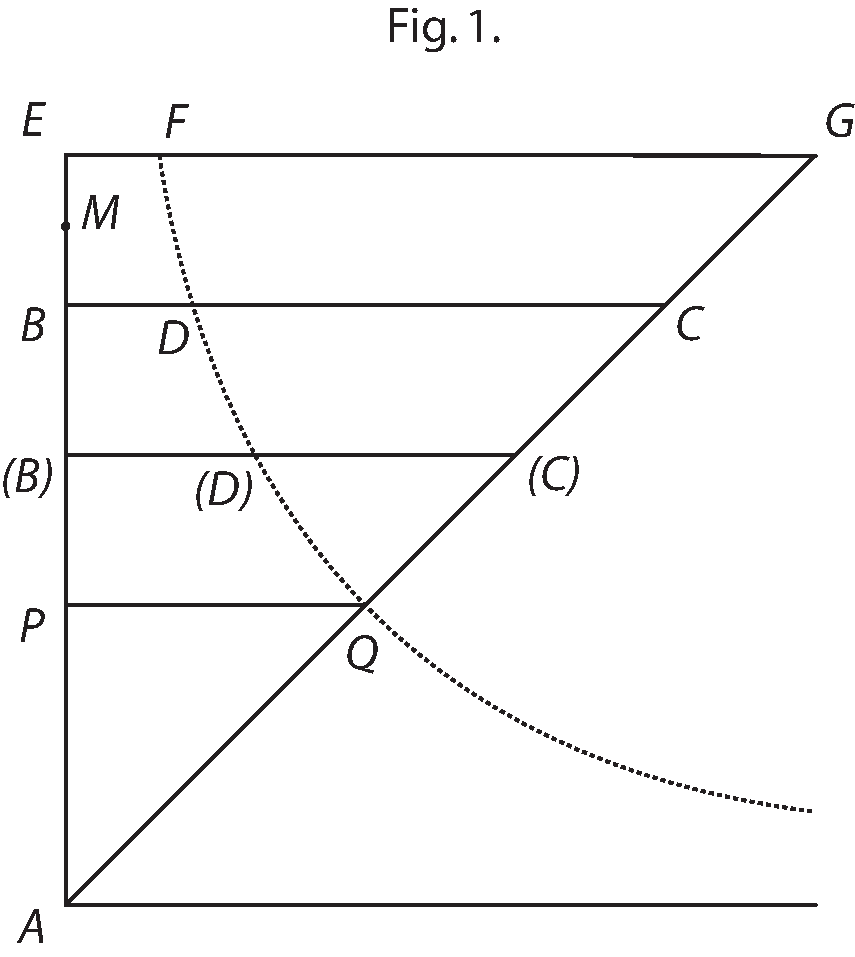
\includegraphics[width=0.4\textwidth]{images/lh0350911_002r-d1.pdf}
  %   \centering
     %[\textit{Fig. 1}] % \caption{Bildbeschreibung}
 %\end{wrapfigure}

%\begin{wrapfigure}{l}{0.4\textwidth}
  %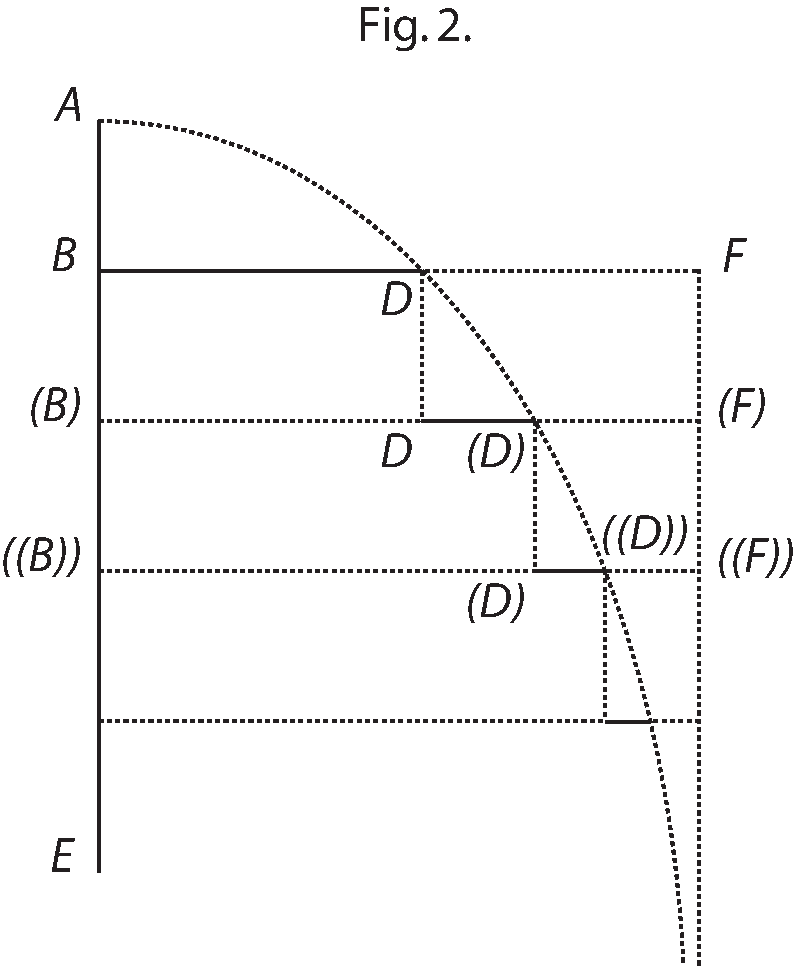
\includegraphics[width=0.2\textwidth]{images/lh0350911_002r-d2.pdf}
    % \centering
    % [\textit{Fig. 2}] % \caption{Bildbeschreibung}
 %\end{wrapfigure}
%
%\vspace{2mm}
\noindent
%\vspace{-6mm}
\begin{minipage}[t]{0.5\textwidth}
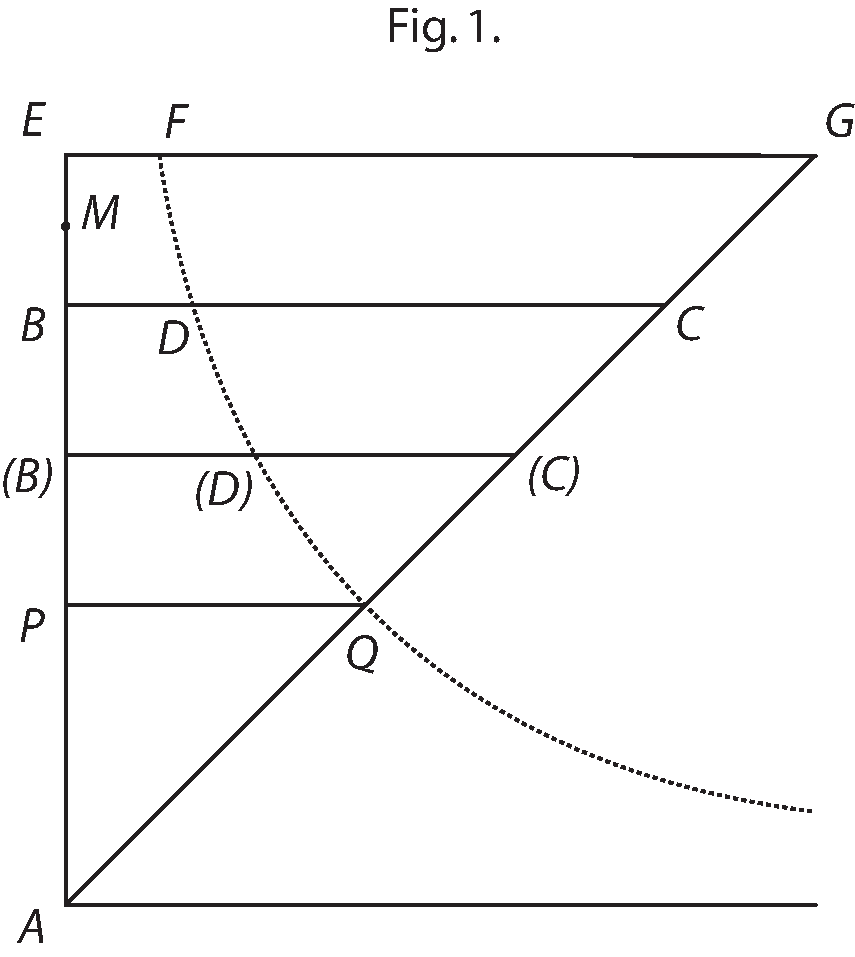
\includegraphics[trim = 0mm 0mm 0mm 17mm, clip, width=0.98\textwidth]{images/lh0350911_002r-d1.pdf}
\end{minipage}
\hspace*{5mm}
\vspace*{0.5mm}
\begin{minipage}[t]{0.5\textwidth}
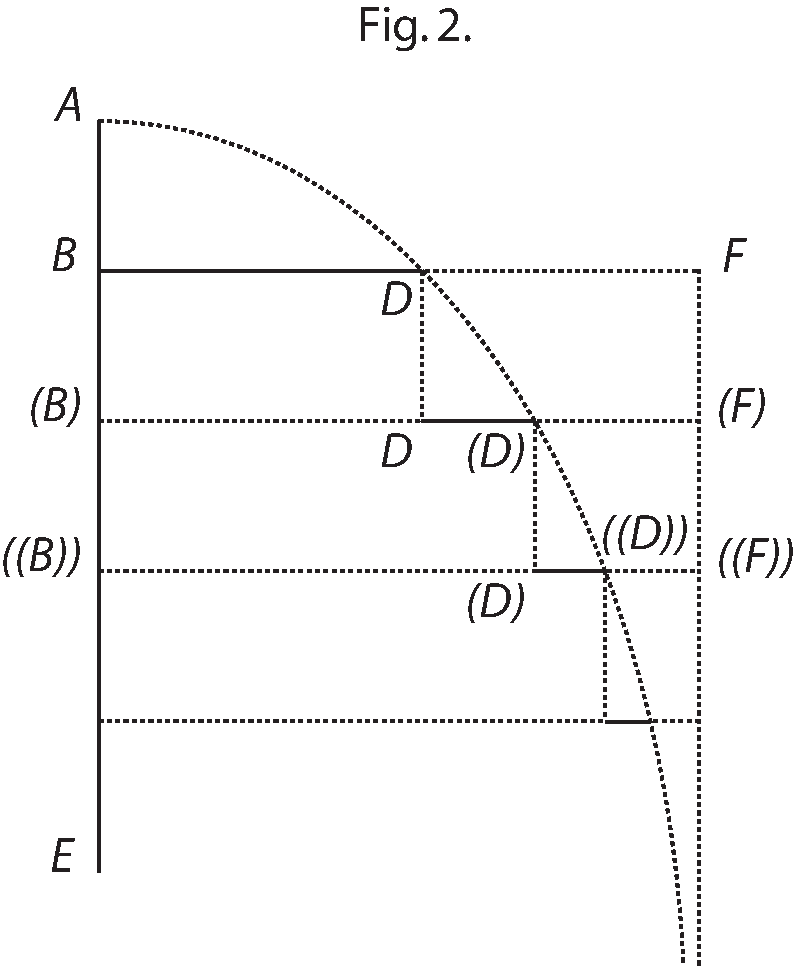
\includegraphics[trim = 0mm 0mm 0mm 10mm, clip, width=0.89\textwidth]{images/lh0350911_002r-d2.pdf}
\end{minipage}
%\vspace*{1em}
\hspace*{26mm} [\textit{Fig. 1}]\hspace*{57mm} [\textit{Fig. 2}]
%\vspace*{1em}
\pend
\newpage
\pstart \begin{center} [\textit{Teil 2}] \end{center} \pend 
\count\Bfootins=1000
\pstart
\noindent
Afin\edlabel{035,09,11_002r_Abschr.}
 de faire voir en peu de mots,
\edtext{que le retardement}{\lemma{que}\Bfootnote{\textit{(1)}\ le decroissem \textit{(2)}\ le retardement \textit{L}}}
uniforme selon les lieux peut avoir lieu dans le calcul du frottement,
conceuuons \edtext{que le frottement}{\lemma{que le}\Bfootnote{\textit{(1)}\ ressort \textit{(2)}\ frottement \textit{L}}}
dans les corps vient des inegalitez de leur
\edtext{surfaces, $\displaystyle AB$ c'est \`{a} dire}{\lemma{surfaces,}\Bfootnote{%
\textbar\ $\displaystyle AB$ \textit{erg. L} \textbar\ %
\textit{(1)}\ et %
\textit{(2)}\ c'est \`{a} dire \textit{L}}}
de quelques eminences ou
\edtext{pointes, $\displaystyle P$ qui se peuuent plier jusqu'\`{a} $\displaystyle p$ pour donner passage}{\lemma{pointes, $\displaystyle P$}\Bfootnote{\textit{(1)}\ qui se plient en $\displaystyle a$\
\textit{(a)}\ \`{a} l'\
\textit{(b)}\ \`{a}\
\textit{(c)}\ ou $\alpha$\
\textit{(d)}\ \`{a} l'entour du centre $\displaystyle B.$
\textit{(2)}\ qui se\
\textit{(a)}\ plient en $\displaystyle p.$\ \`{a} l'entour du centre\
\textit{(aa)}\ $\displaystyle P$\
\textit{(bb)}\ $\displaystyle C$\
\textit{(b)}\ peuuent plier jusqu'\`{a} $\displaystyle p$\ \textbar\ \`{a} l'entour du centre $\displaystyle C$ \textit{gestr.}\ \textbar\ pour\
\textit{(aa)}\ faire place\
\textit{(bb)}\ donner passage \textit{L}}}
au mobile $\displaystyle M$
quoyqu'ils se remettent par
%\begin{wrapfigure}[8]{l}{0.45\textwidth}
%     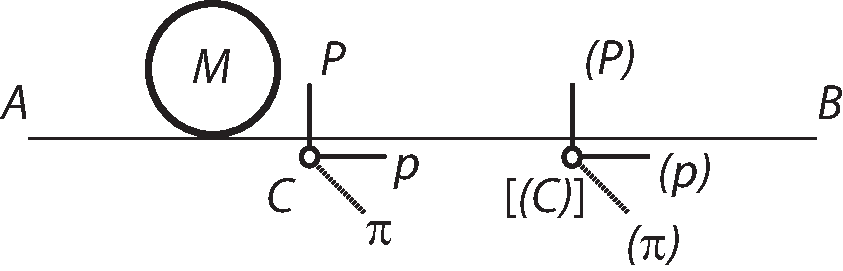
\includegraphics[trim = 0mm -3mm 0mm 0mm, clip, width=0.45\textwidth]{images/lh0350911_002r-d3.pdf}
%    \centering
%     \edtext{[\textit{Fig. 3}]}{\lemma{ [\textit{Fig. 3}]} \killnumber\Bfootnote{$\ \ \displaystyle (C)$ \textit{erg. Hrsg.}}}\\
%     % \caption{Bildbeschreibung}
%  \end{wrapfigure}
leur propre ressort\protect\index{Sachverzeichnis}{ressort},
quand le mobile est pass\'{e}. Cela pos\'{e}, il est manifeste que le mobile
perd autant de sa force\protect\index{Sachverzeichnis}{force}
qu'il en a communiqu\'{e} au ressort ou \`{a} la
\edtext{pointe $\displaystyle P$}{\lemma{pointe}\Bfootnote{\textit{(1)}\ $\displaystyle CP$ \textit{(2)}\ $\displaystyle P$. \textit{L}}}.
Et comme la force est
\edtext{compos\'{e}e de la pesanteur}{\lemma{compos\'{e}e}\Bfootnote{\textit{(1)}\ de la grandeur \textit{(2)}\ de la pesanteur \textit{L}}}
du corps, et de sa vitesse\protect\index{Sachverzeichnis}{vitesse},
il est manifeste que le corps $\displaystyle M$ demeurant le m\^{e}me,
la deminution de sa force, ne \setline{11}sera que celle de la vitesse.
\pend
\vspace{1em}
\pstart \noindent \centering
     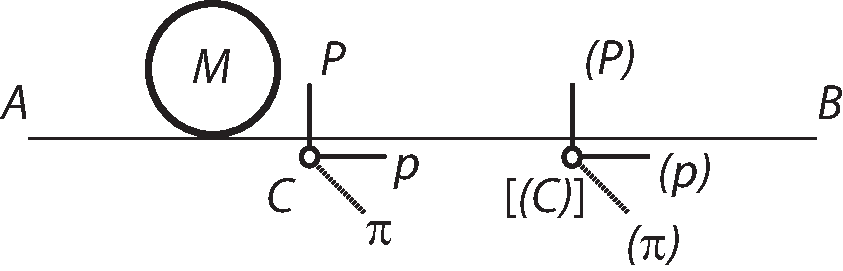
\includegraphics[trim = 0mm -3mm 0mm 0mm, clip, width=0.5\textwidth]{images/lh0350911_002r-d3.pdf}\\
    \centering
     \edtext{[\textit{Fig. 3}]}{\lemma{ [\textit{Fig. 3}]} \killnumber\Bfootnote{$\ \ \displaystyle (C)$ \textit{erg. Hrsg.}}}
     % \caption{Bildbeschreibung}
  \pend
  \vspace{1em}
%\newpage
\count\Bfootins=1000
\pstart
Or \setline{10}supposons \`{a} present que
\edtext{le Mobile $\displaystyle M$}{\lemma{le}\Bfootnote{\textit{(1)}\ corps \textit{(2)}\ Mobile $\displaystyle M$ \textit{L}}}
continue son mouuement sur la m\^{e}me surface,
quoyque avec une vitesse diminu\'{e}e,
et qu'il rencontre une autre pointe $\displaystyle (P)$ semblable en tout \`{a} la premiere,
parce que nous supposons la dite surface \'{e}galement \^{a}pre par tout:
alors le mobile pourveu qu'il ait
\edtext{encor assez de}{\lemma{encor}\Bfootnote{\textit{(1)}\ \`{a} ce d \textit{(2)}\ assez de \textit{L}}}
force, ne laissera pas de plier encor de m\^{e}me la
\edtext{seconde}{\lemma{}\Bfootnote{seconde \textit{erg. L}}}
pointe $\displaystyle (C)(P)$ pour se faire
\edtext{passage.\\
\hspace*{7,5mm}Or pour faire passage au mobile,
(que nous supposons bien uni pour la facilit\'{e} de l'imagination, ne donnant les inegalitez qu'\`{a} la surface du corps sur le quel il marche)
il suffit}{\lemma{passage.}\Bfootnote{\textit{(1)}\ Or pour se faire passage il\ \textit{(a)}\ fau\ \textit{(b)}\ suffit tous \textit{(2)}\  Or pour faire passage\ \textit{(a)}\ \`{a} la pointe\ \textit{(b)}\ au mobile, [...] il suffit \textit{L}}}
que la pointe soit pli\'{e}e jusqu'\`{a}
\edtext{ce qu'elle}{\lemma{ce}\Bfootnote{\textit{(1)}\ que la dite pointe\ \textit{(a)}\ $\displaystyle cP$ ou $\displaystyle (C)(P)$\ \textit{(b)}\ $\displaystyle Cp$ \textit{(2)}\ qu'elle \textit{L}}}
soit devenue parallele \`{a} la surface
(ou si elle est courbe, au
\edtext{plan touchant}{\lemma{plan}\Bfootnote{\textit{(1)}\ tangent \textit{(2)}\ touchant \textit{L}}}) $\displaystyle AB$.%
% [2~v\textsuperscript{o}]
% \pend